% Created 2016-05-26 Thu 13:07
\documentclass[11pt]{article}
\usepackage[utf8]{inputenc}
\usepackage[T1]{fontenc}
\usepackage{fixltx2e}
\usepackage{graphicx}
\usepackage{grffile}
\usepackage{longtable}
\usepackage{wrapfig}
\usepackage{rotating}
\usepackage[normalem]{ulem}
\usepackage{amsmath}
\usepackage{textcomp}
\usepackage{amssymb}
\usepackage{capt-of}
\usepackage{hyperref}
\author{Mikael Svahnberg}
\date{\today}
\title{}
\hypersetup{
 pdfauthor={Mikael Svahnberg},
 pdftitle={},
 pdfkeywords={},
 pdfsubject={},
 pdfcreator={Emacs 25.1.50.1 (Org mode 8.3.4)}, 
 pdflang={English}}
\begin{document}

\tableofcontents

\section{2 Object-Oriented Modelling - Modelling Structure}
\label{sec:orgheadline3}
\subsection{Task}
\label{sec:orgheadline1}
Draw a conceptual model for the following fragment of the problem domain.

In the Country lives a community of persons - workers and students.
Every person has a name, personal number and address.

The address consists of the name of the town, the name of the street and the number of the
apartment/flat (such as Stockholm, Vasa Street, 25).

Every person can have a number of mobile phones.

Every phone can have 1 or two phone cards. Every card has the PIN code (used to identified the
legal usage of the card when the card is inserted into the phone) and the call number (the number
that is used for calling).

There two types of phones – touch screen phones and
To the keypad phones the microphone can be attached as an external device.

A person can work in a company. A person can work in no more than 4 companies, but a company
may employ any number of workers.

When employed, a person gets a salary, may be different in different working places.
The salary consists of a basic salary, extra salary and bonus.

At a given moment a person can be unemployed.

\subsection{Solution}
\label{sec:orgheadline2}
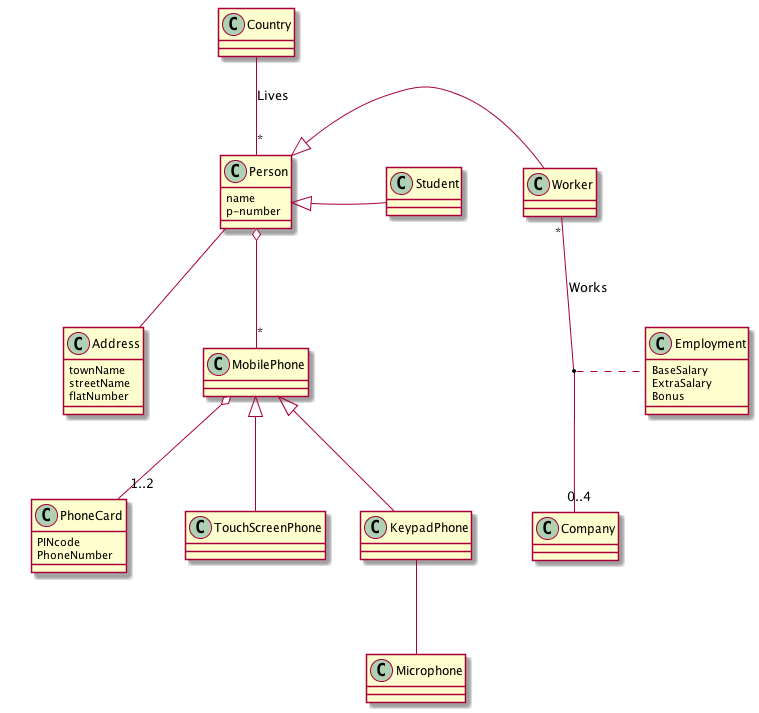
\includegraphics[width=.9\linewidth]{FConceptual-20160109_SOLVED.png}

\section{2.1 Modelling Behaviour}
\label{sec:orgheadline6}
\subsection{Task}
\label{sec:orgheadline4}
A (rather very special) Digital Watch can display the time -- hours and minutes.

When the watch is created the watch displays time - hours and minutes,
and they both are set to zero.

Both the hours and minutes can be adjusted.
This is dine using two buttons attached to the watch – A button and B button.

When the watch is displaying the time - steady, non-blinking hours and minutes,
and the B button is pressed - nothing happens and the watch continues to display the time.
But when the A button is pressed then the watch starts to display only blinking hours
and the hours can be change by pressing the B button.
Each pressing of the button B increasing the hours by one.

Then when pressing the A button the watch starts to display only blinking minutes
and then the button B can be pressed to change the minutes.
Each pressing the button B increases the minutes by one.

Then when the button A is pressed the watch stats to display the newly set time
\begin{itemize}
\item steady, non-blinking hours and minutes. When the button A is pressed it starts to blinking hours etc
\end{itemize}

Provide an UML model describing the watch - both the structure and behaviour of the watch.
\subsection{Solution}
\label{sec:orgheadline5}
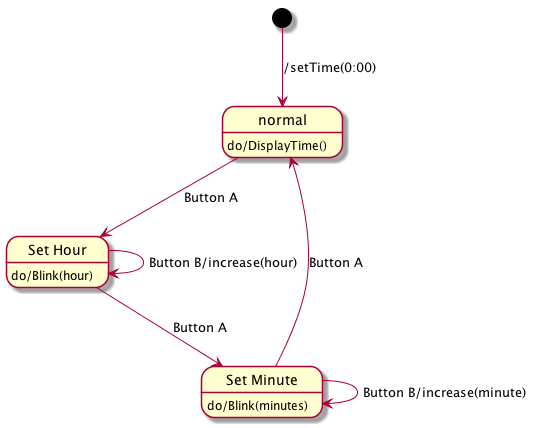
\includegraphics[width=.9\linewidth]{FState-20160109-SOLVED.png}

\section{3 Object Oriented Design}
\label{sec:orgheadline18}
\subsection{Task}
\label{sec:orgheadline7}
Bank Terminal

Bank Terminal is a device from which you can perform a number of operations on your bank
account.

It is situated in a number of places around the town and has a direct telecommunication
connection with a bank. It has a screen to display information and a number of buttons.

At the Bank Terminal you can withdraw money from you account.

Before you decide on how much you want in cash you can check how much money is
available on the account. You can also make a choice on the values of the banknotes (paper
money) you want the requested money be delivered – 500, 100, and 50.

The Bank Terminal will try to deliver the money as close to your request as possible.

You will not get the money if the requested amount is greater than the amount available on
the account or if there is not enough money in the terminal container.

When the terminal is running out of money the terminal maintenance office should be notified.

At the terminal you can also make examination of you account. This includes a look-up of all
operations preformed on the account, printing the actual balance and printing operations
performed. In the last case you can make a choice what operations you want to be printed,
choose the format of the printing and also choose the device on which they will be printed.

To withdraw the money and to examine your account you have to authorize.

For the authorization you have to insert your bank card to a special slot.

A scanner reads the card and asks you to enter PIN code. Then proceeds to the verification
process.

During the verification process the terminal contacts with the bank, providing appropriate
information about the card used for the transaction, and gets a reply if the card is valid.

Then you are asked for a code. If the code is ok you can proceed with the operations
otherwise you are asked to retype the code. After three unsuccessful trials your card is kept.

The terminal contacts the bank using fibre cable connection if there is a need to obtain or to
update the information about your account.
\subsection{Solution}
\label{sec:orgheadline17}
\subsubsection{Actors}
\label{sec:orgheadline8}
\begin{itemize}
\item Customer
\item Bank
\item Maintenance Office
\end{itemize}
\subsubsection{Use Cases}
\label{sec:orgheadline9}
\begin{itemize}
\item Withdraw Money
\item Examine Account
\item Authorisation
\item Out of Money
\end{itemize}
\subsubsection{Use Case Diagram}
\label{sec:orgheadline10}
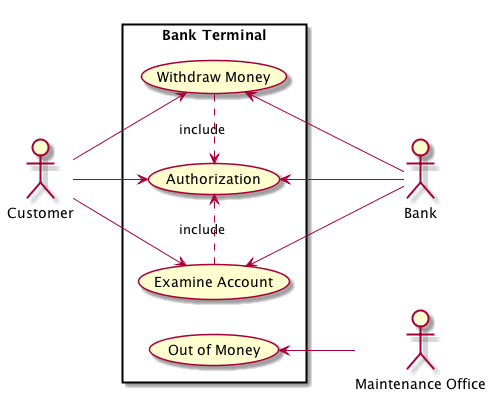
\includegraphics[width=.9\linewidth]{FUCD-20160109_SOLVED.png}

\subsubsection{Extended Use Case \texttt{WithdrawMoney}}
\label{sec:orgheadline11}
Use Case: Withdraw Money

Primary Actor: Customer

Actors: Bank

Preconditions:
\begin{itemize}
\item Customer is a customer at the bank
\item There is money in the bank terminal
\end{itemize}

Postconditions:
\begin{itemize}
\item Customer walks away with cash in hand
\item The customers account is accordingly updated
\end{itemize}

Description: A customer authenticates themselves against the bank, and selects how much money they want to withdraw and in what types of banknotes. The system updates the account (if there is enough money) and gives the money to the customer.

\begin{scriptsize}
Main Flow of Events:
\begin{center}
\begin{tabular}{ll}
Actor & System\\
\hline
1. Customer \emph{Authorises} themself to the machine & 2. Initiate use case \uline{Authorisation}\\
3. Customer \emph{Checks} how much money is available & 4. System displays the amount of money on the account.\\
5. Customer decides how much money they want & \\
6. Customer decides what banknotes they want & 7. System verifies that there are sufficient funds in the account.\\
 & 8. System subtracts desired amount from account.\\
 & 9. System dispenses money (according to the preferred banknotes).\\
 & 10. System returns card.\\
\hline
\end{tabular}
\end{center}
\end{scriptsize}

Alternative Flows:
\begin{itemize}
\item 2. Customer fails to authorise themselves correctly. The transaction is aborted.
\item 7. There are not enough money in the account. The transaction is aborted and an error message is shown.
\item 9. The desired banknotes are not available. The system dispenses other banknotes.
\item 9. There is not enough money in the machine. The transaction is aborted and the system initiates the \uline{out of money} use case.
\end{itemize}

\subsubsection{Conceptual Model}
\label{sec:orgheadline12}
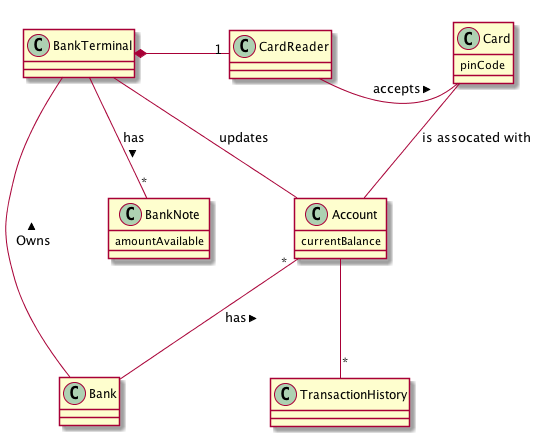
\includegraphics[width=.9\linewidth]{FConceptual2_20160109_SOLVED.png}

\subsubsection{System Operations}
\label{sec:orgheadline13}
Authorise(pin,cardNumber)
CheckAccount()
WithdrawAmount(theAmount)
setPreferredBankNotes(theNoteType)   
\subsubsection{Signature}
\label{sec:orgheadline14}
\texttt{void WithdrawAmount(int theAmount)}
\subsubsection{Collaboration Diagram}
\label{sec:orgheadline15}
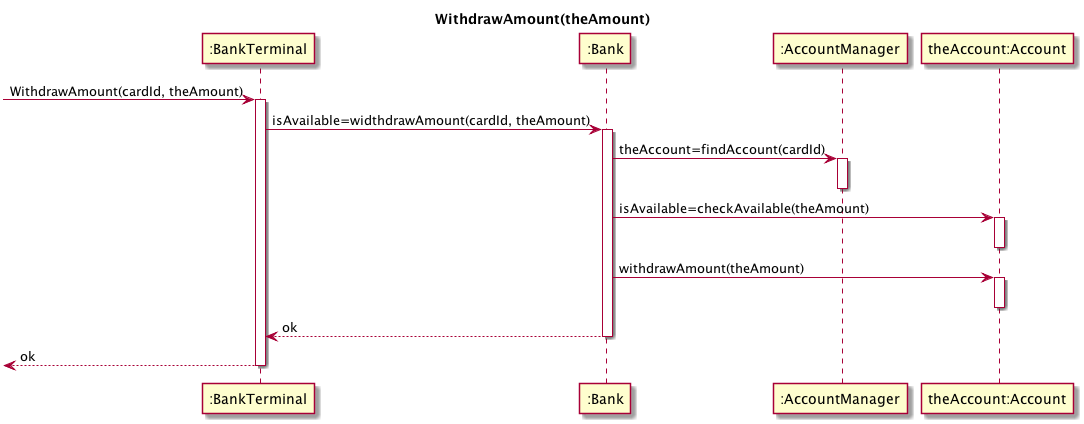
\includegraphics[width=.9\linewidth]{FCollaboration-20160109_SOLVED.png}

\subsubsection{{\bfseries\sffamily TODO} Contract}
\label{sec:orgheadline16}
\end{document}